\section{Podsumowanie i testy stacji}

Testy stacji stanowiły testy części radiowej i konstrukcyjnej. W ramach grantu kupiono balon na misję balonową, aby wraz z układem z poprzedniego grantu przetestować łącze radiowe w praktycznych warunkach.

\subsection{Test współpracy z oprogramowaniem Orbitron}

W celów testu wyznaczyliśmy w programie symulowany przelot stacji ISS w okolicach Warszawy i włączyliśmy nasz sterownik do wodzenia anteną za stacją ISS będącą najszybciej poruszającym się obiektem na bliskiej orbicie.

Oprogramowanie zadziałało poprawnie i stacja była sterowana za pośrednictwem komputera. W tym teście okazało się, że stacja ISS przy bliskim przelocie jest znacząco zbyt szybko poruszającym się obiektem dla naszego rotora. Rotor nadążął za zmianami w płaszczyźnie elewacji, ale zmiany azymutalne były zbyt duże. Jak wcześniej wspomniano, można przyspieszyć obroty zwiększając napięcie, ale ogólnie nie przewidywaliśmy śledzenia tak szybkich obiektów. Na zakończenie kilkunastosekundowego testu zrobiliśmy pomiar zewnętrznym kompasem. Jest to przedstawione na rysunku \ref{kompas}.

Test orientacji w płaszczyźnie azymutu wykazał błąd na poziomie $\pm 3^o$, ze względu na niską dokładność użytego kompasu w module. Z drugiej strony potencjalna rozdzielczość rotora w jednostce na impuls enkodera wynosi $0.02^o$ w płaszczyźnie elewacji i $0.2^o$ w płaszczyźnie azymutu dzięki wolnym obrotom. W związku z tym dodaliśmy opcję ręcznego wprowadzenia kalibracji orientacji z komputera jeśli zajdzie potrzeba uzyskania większej dokładności.

Wykonaliśmy test obrotu dookoła, aby sprawdzić czy sterownik steruje poprawnie i nie zerwie kabla sterownika. Rotor poprawnie zaprogramowany nie zerwał kabla i zaczął obracać się w przeciwnym kierunku (o ujemny kąt) aby wykonać pełen obrót.

\begin{figure}[h]
	\centering
		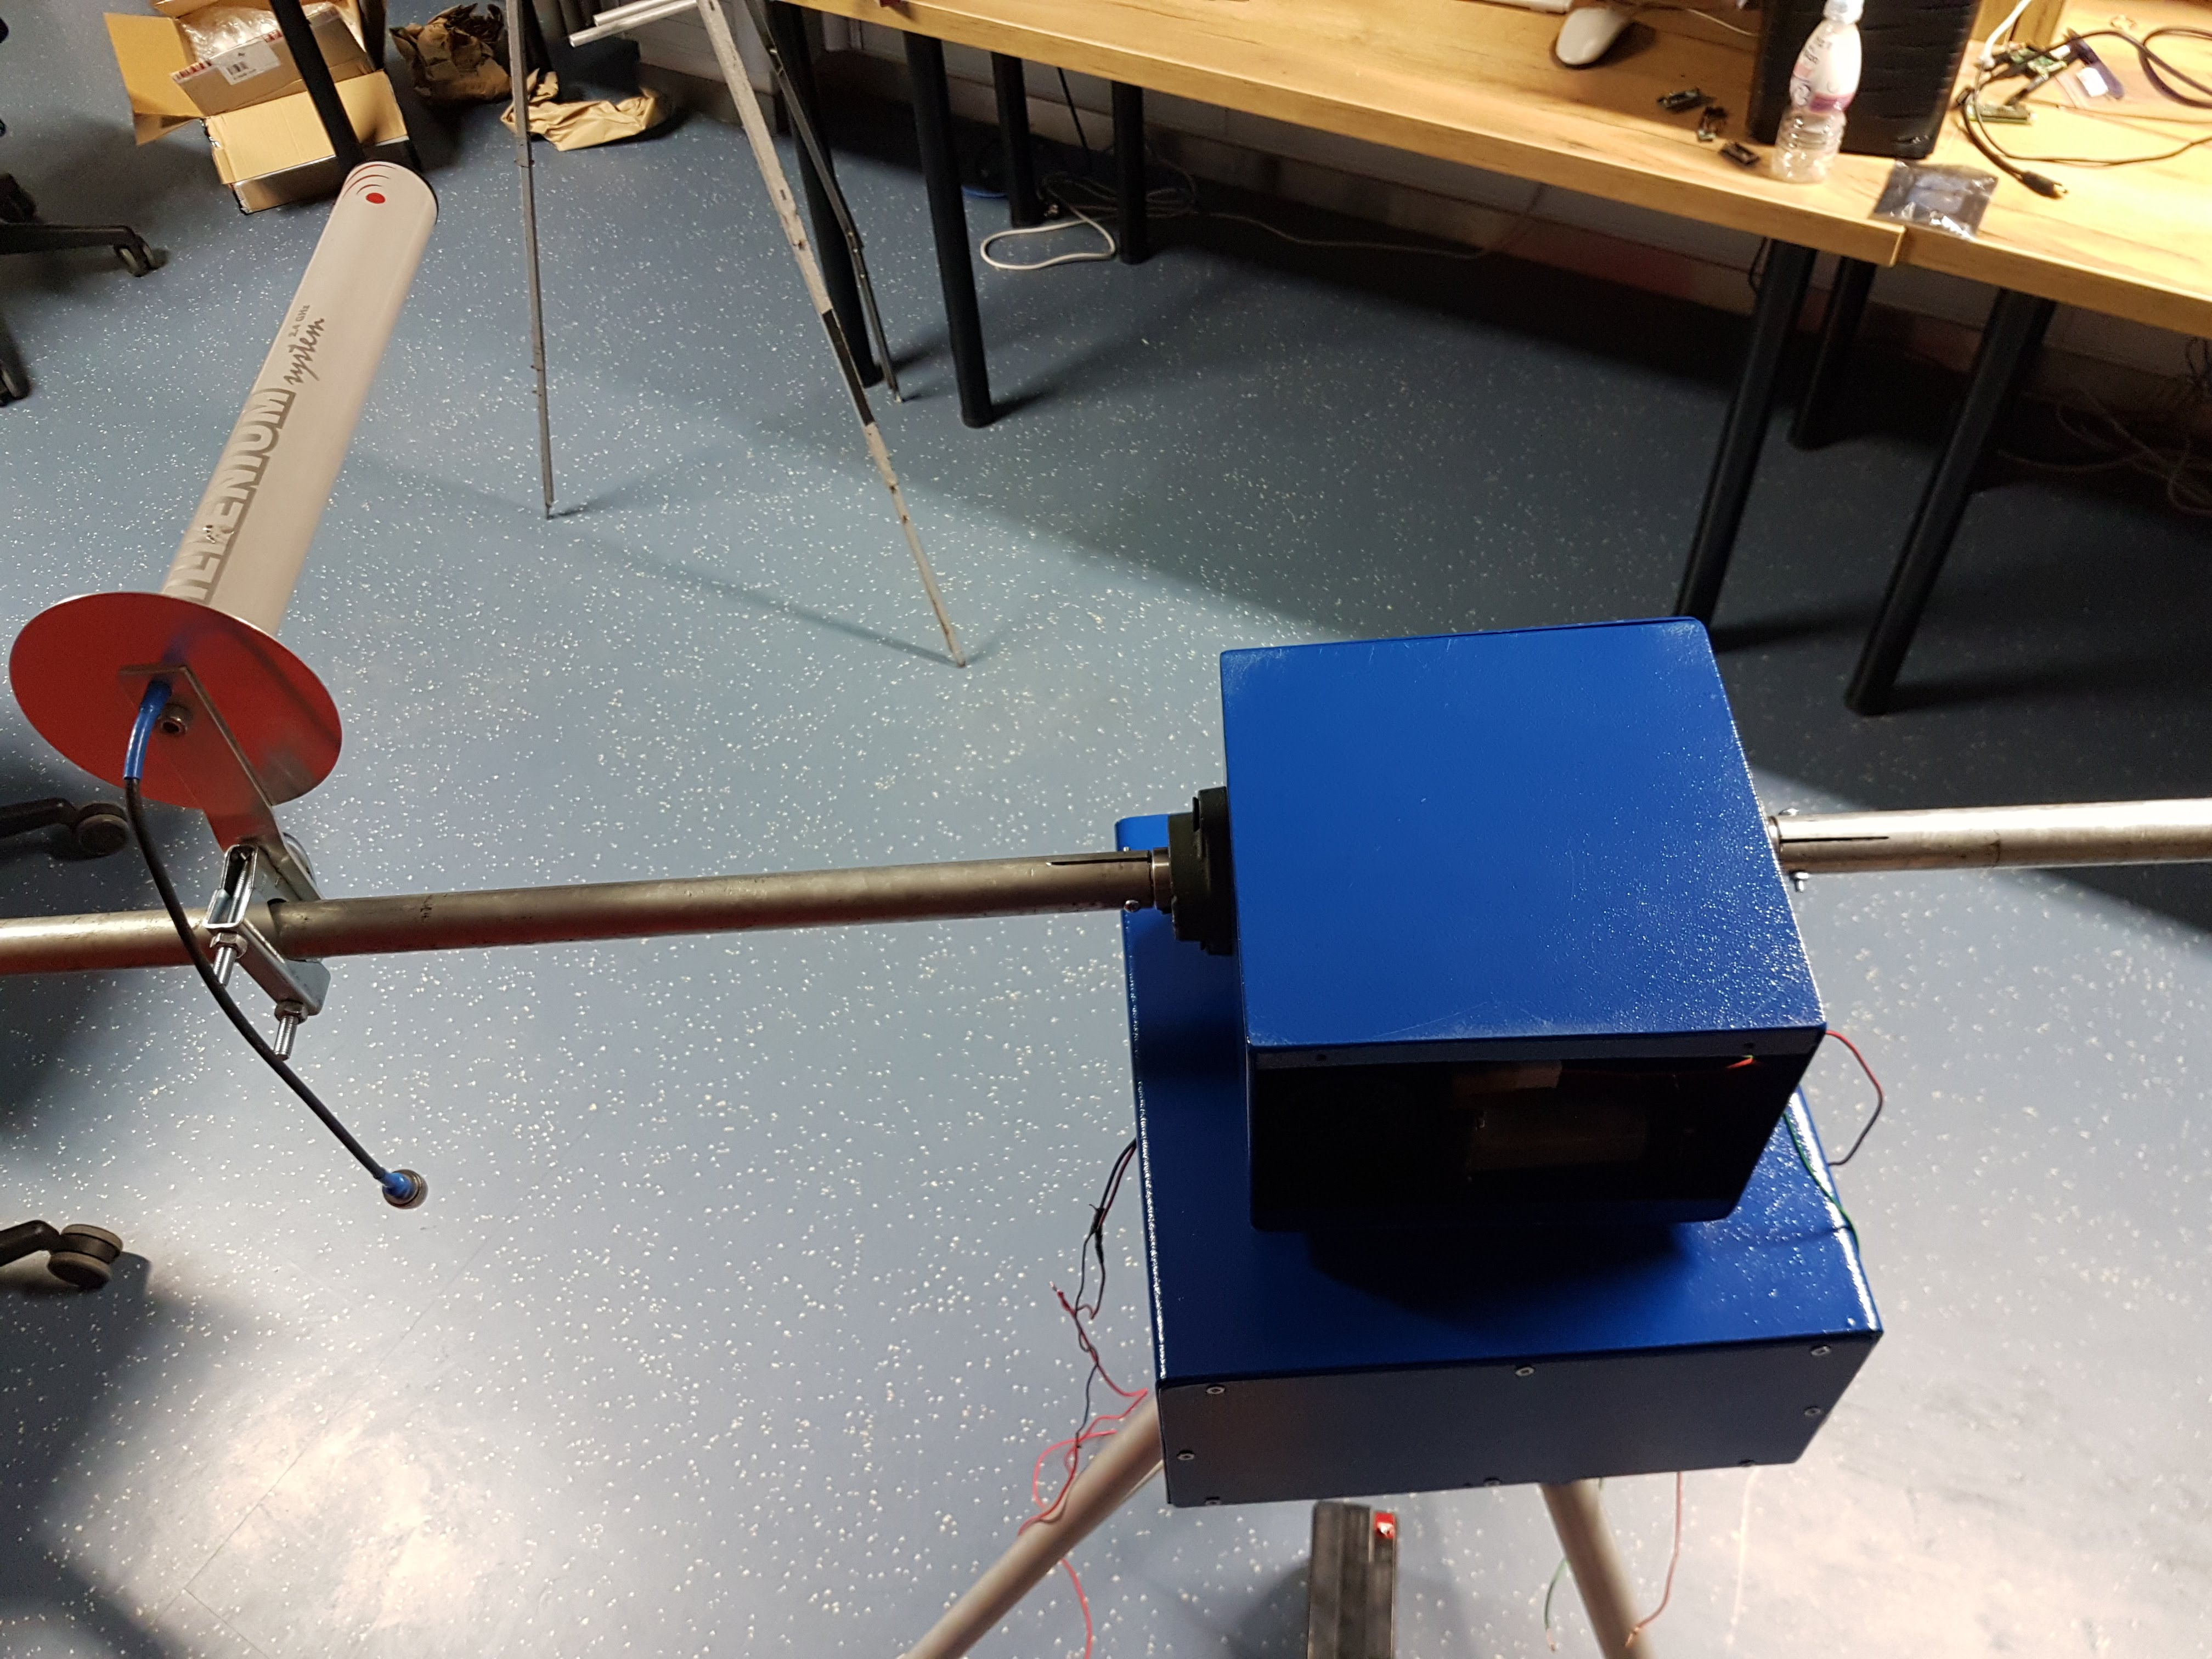
\includegraphics[width=0.7 \textwidth]{testy/antenaS}
	\caption{Antena wskazuje kierunek południowy}	
	\label{fig:antenaS}
\end{figure}

\begin{figure}[h]
	\centering
		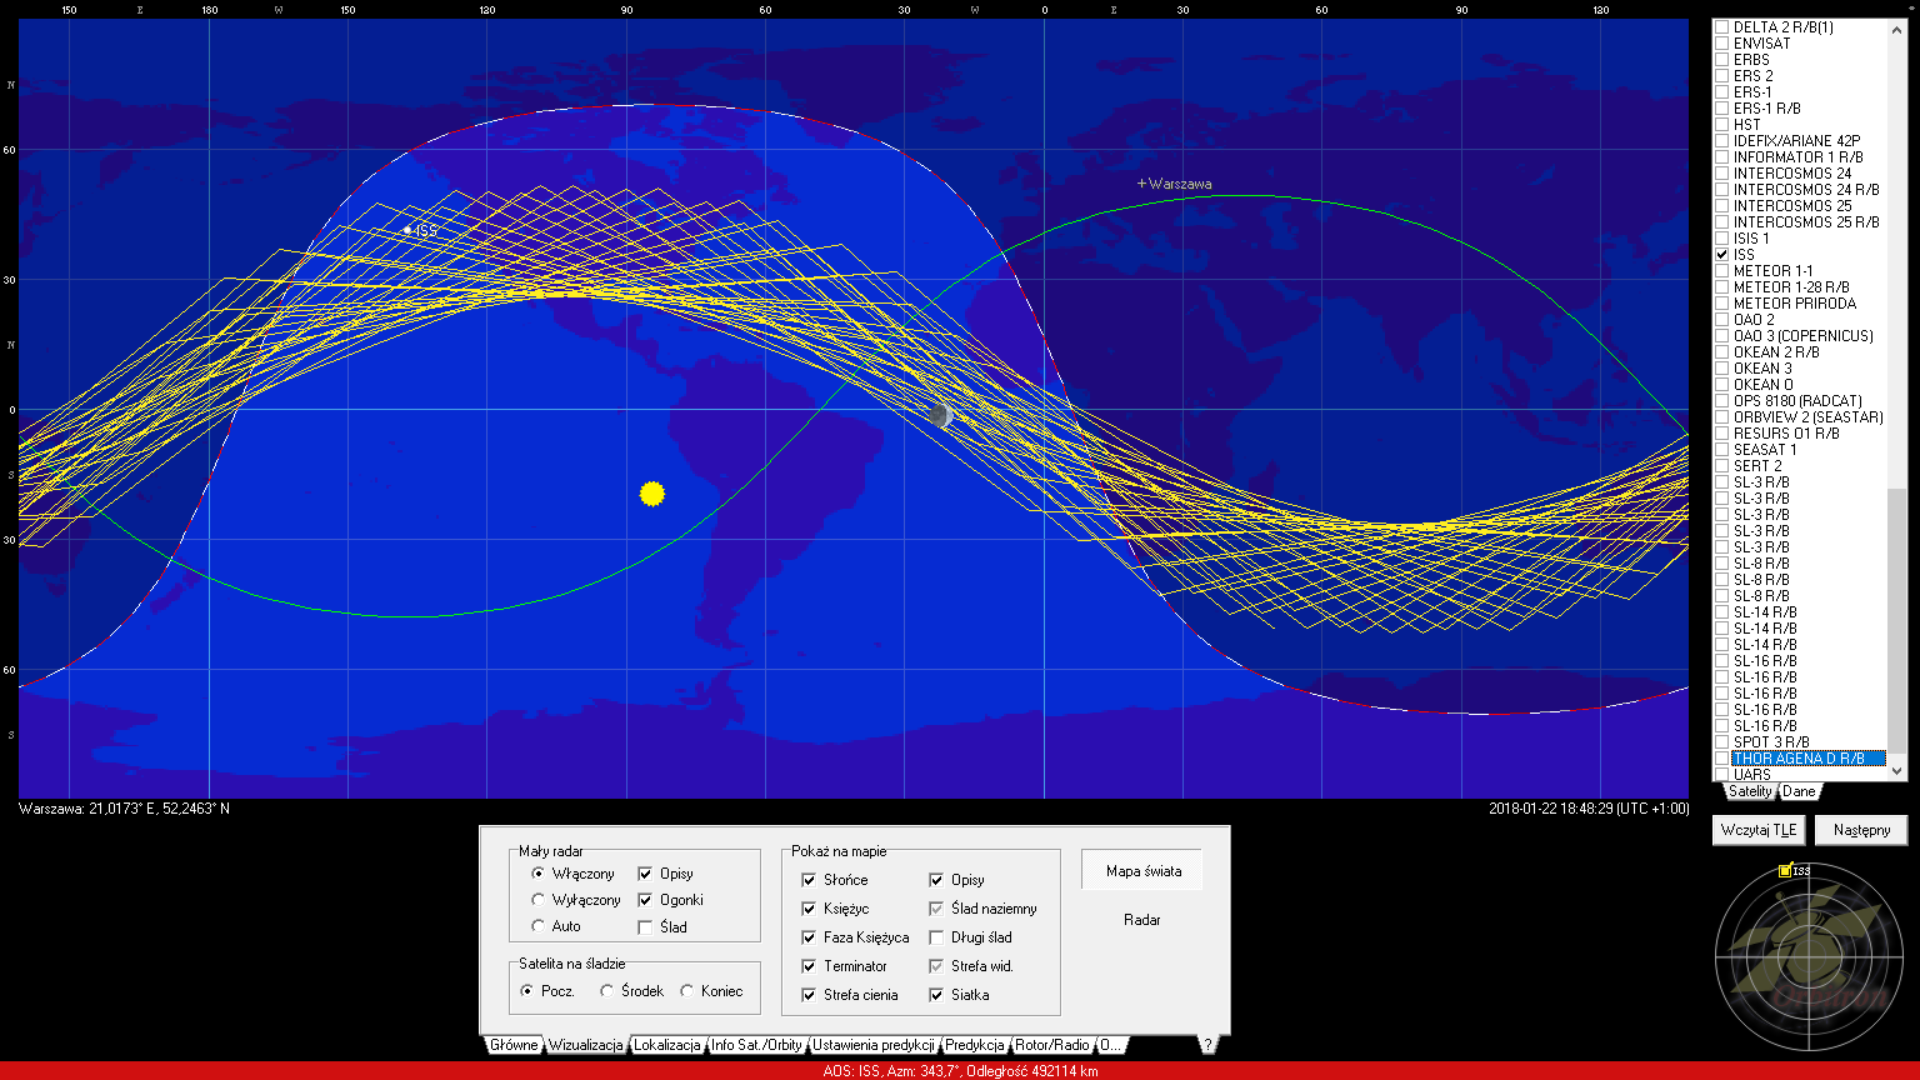
\includegraphics[width=0.7 \textwidth]{testy/pojawia}
	\caption{Satelita ISS pojawia się nad horyzontem}	
	\label{fig:pojawia}
\end{figure}

\begin{figure}[h]
	\centering
		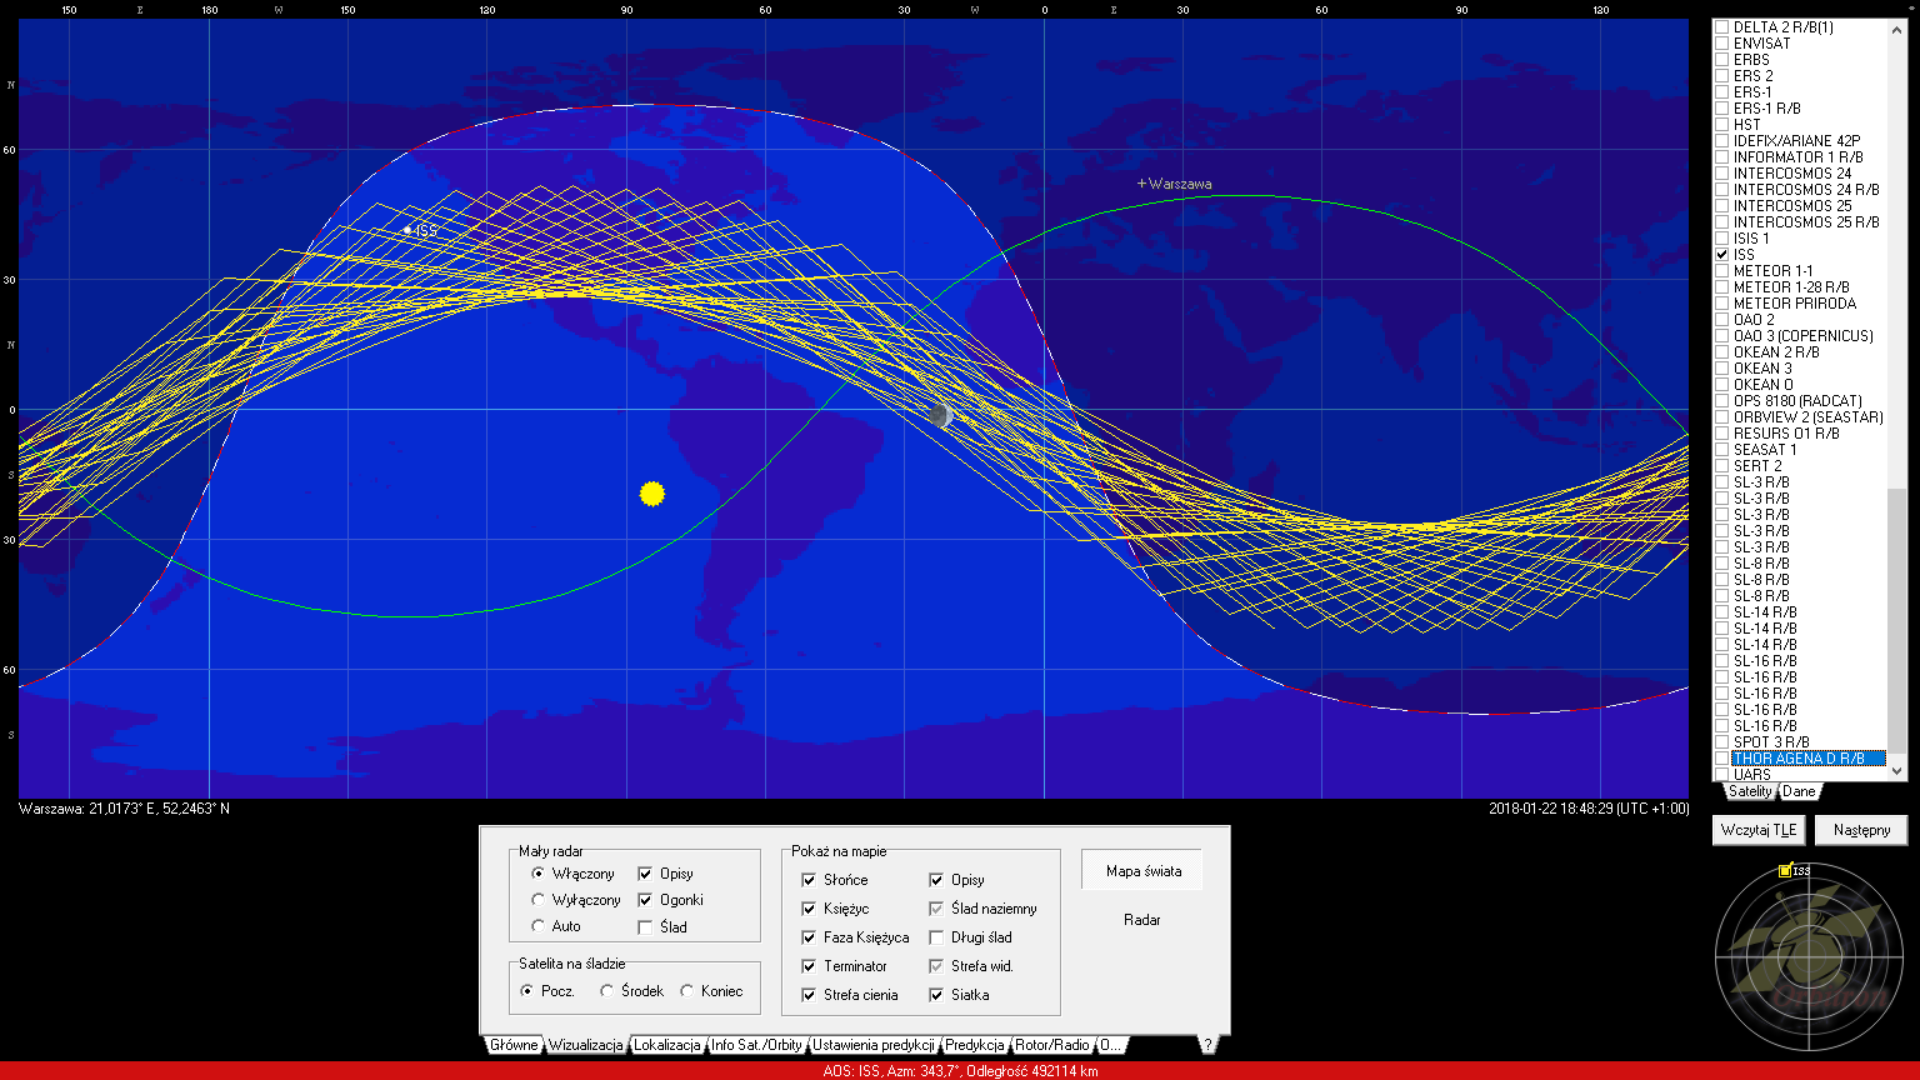
\includegraphics[width=0.7 \textwidth]{testy/pojawia}
	\caption{Satelita ISS pojawia się nad horyzontem}	
	\label{fig:pojawia}
\end{figure}


\begin{figure}[h]
	\centering
		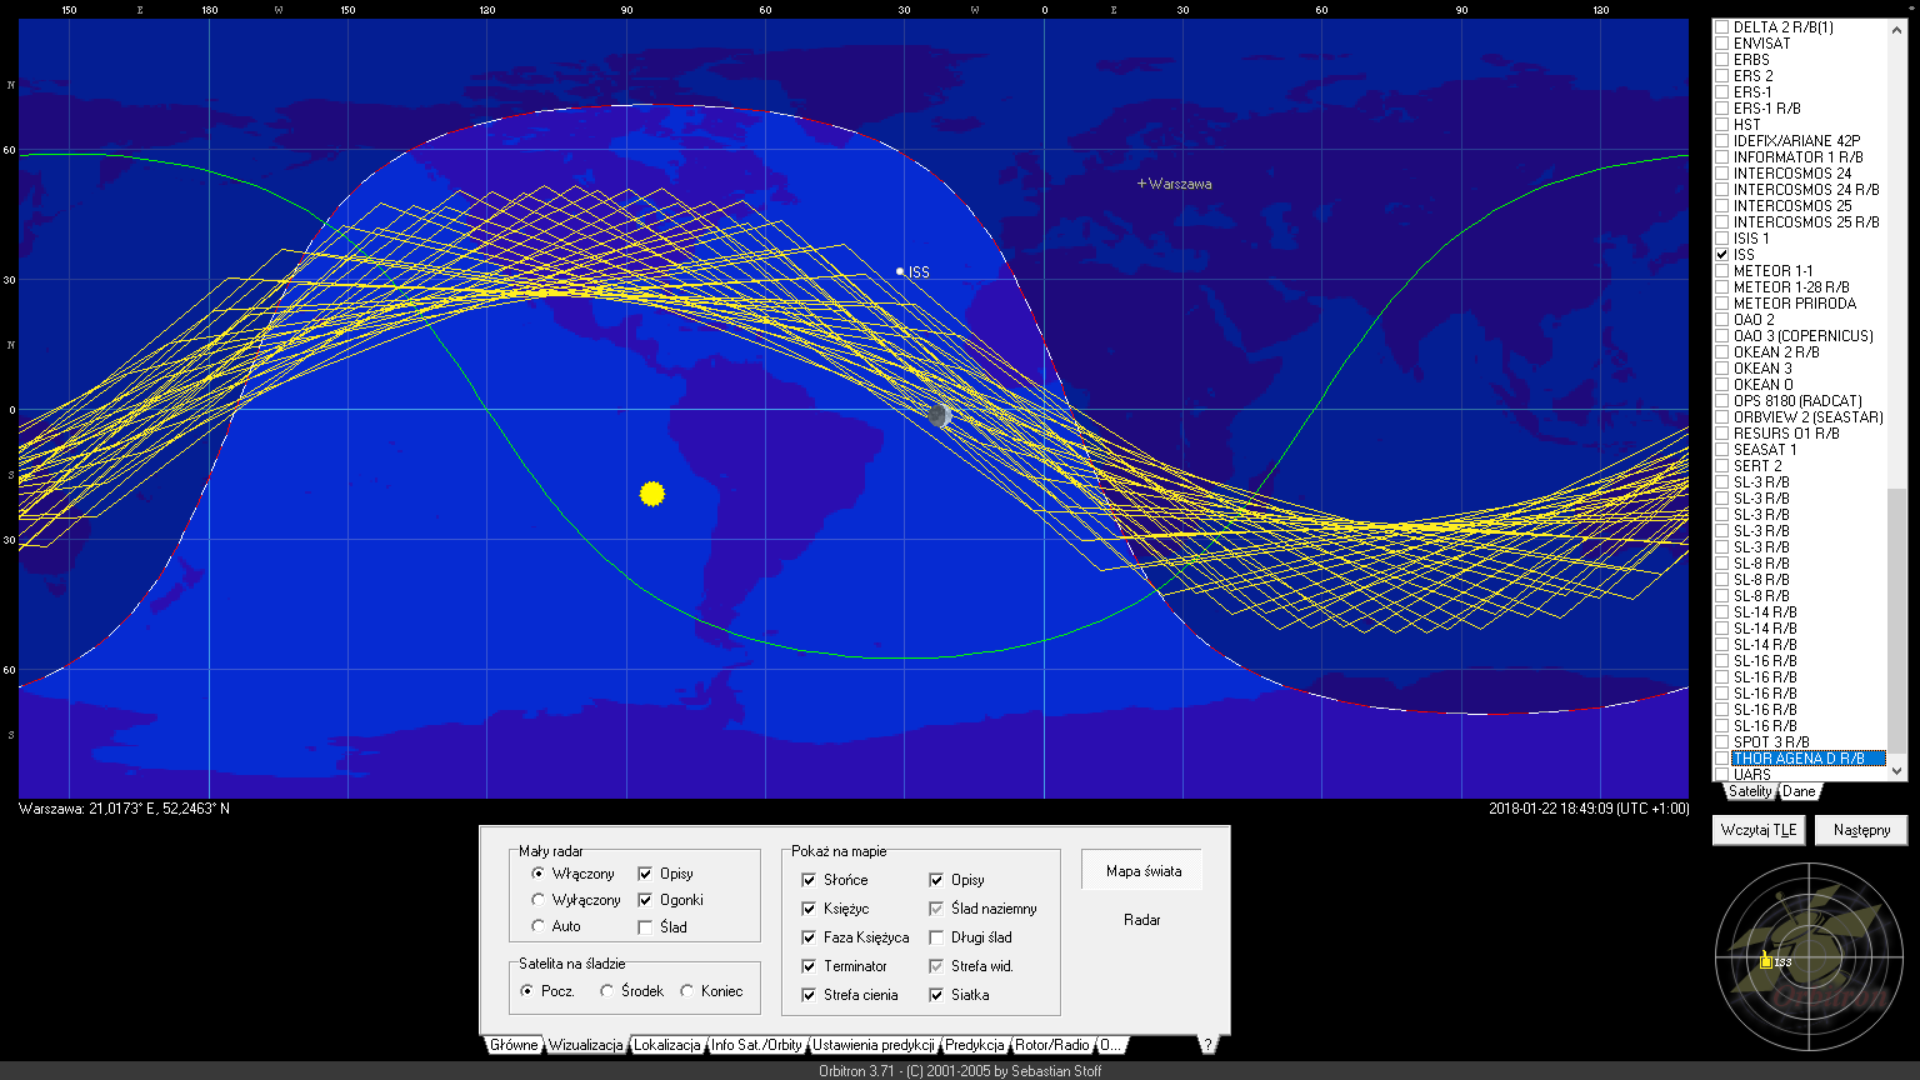
\includegraphics[width=0.7 \textwidth]{testy/zenit}
	\caption{Satelita ISS w zenicie}	
	\label{fig:zenit}
\end{figure}


\begin{figure}[h]
	\centering
		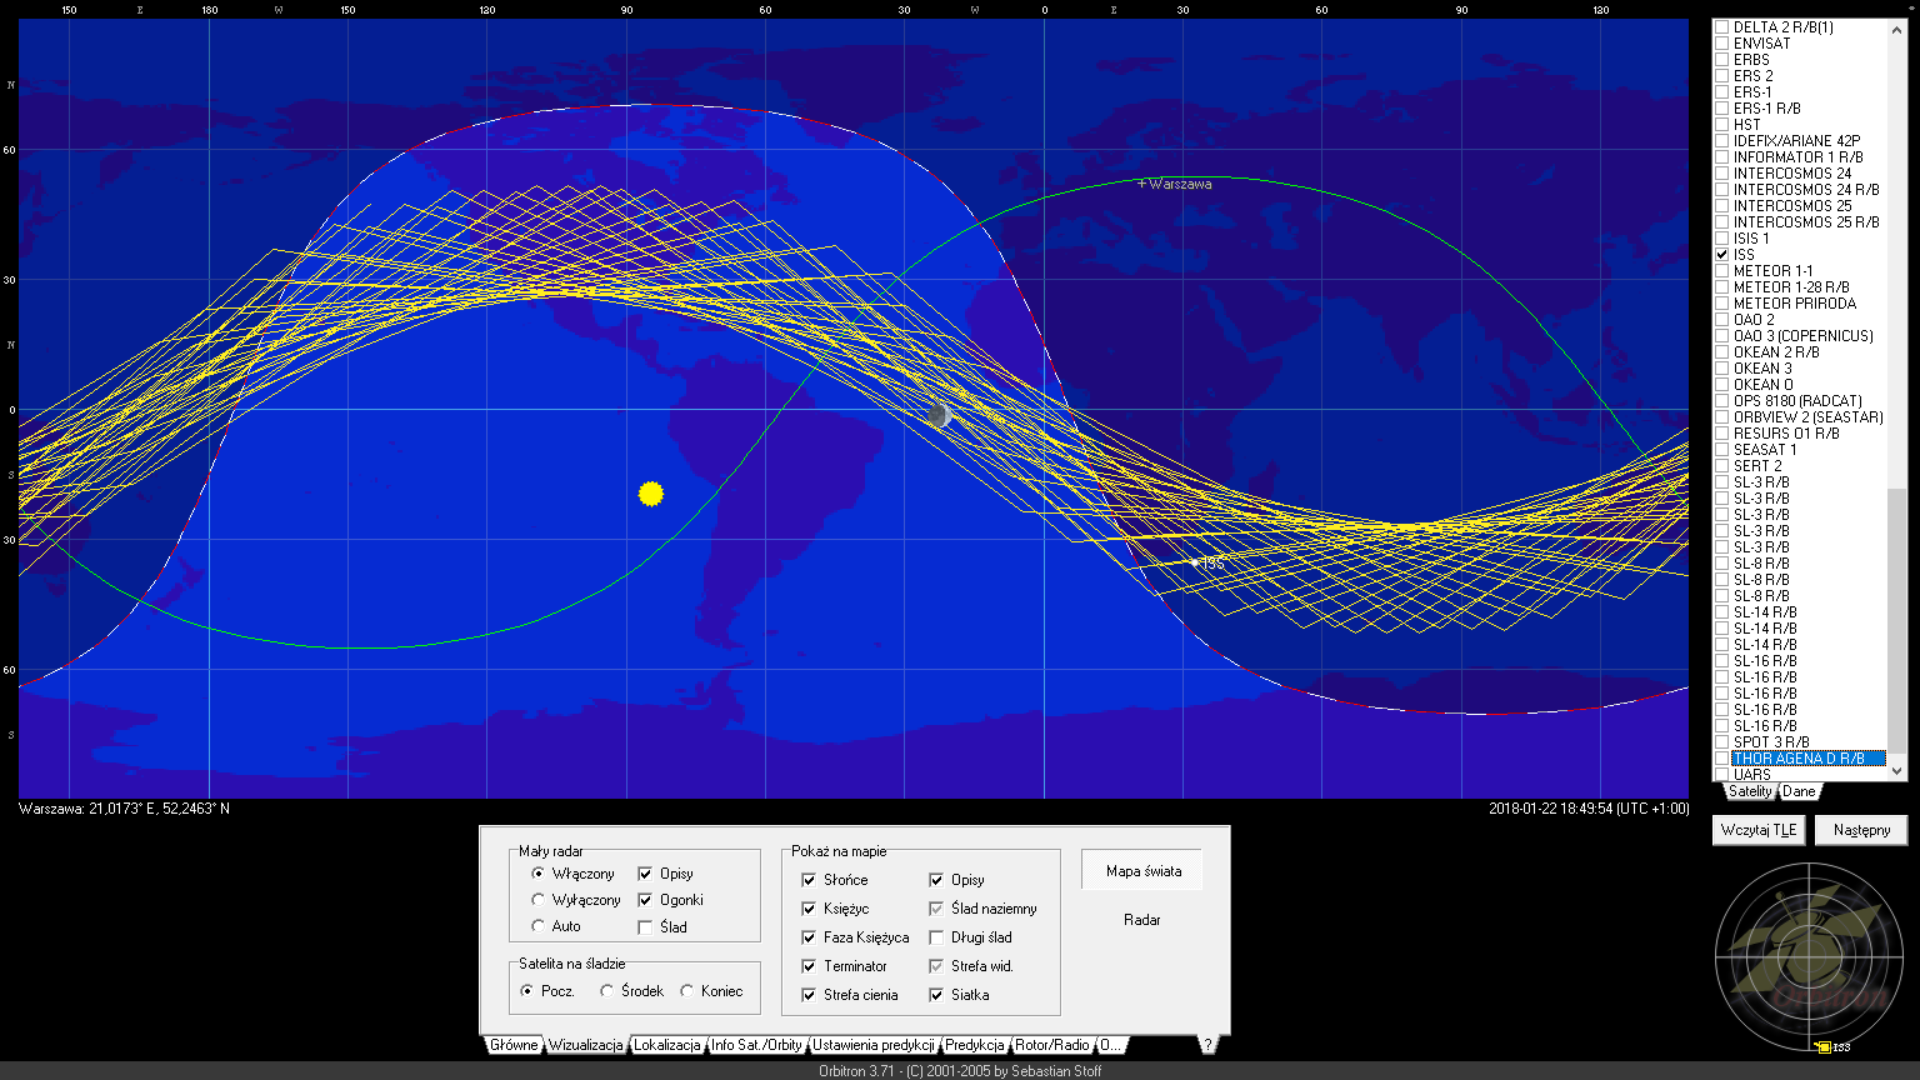
\includegraphics[width=0.7 \textwidth]{testy/znika}
	\caption{Satelita ISS znika za horyzontem}	
	\label{fig:zanika}
\end{figure}


\begin{figure}[!htbp]
 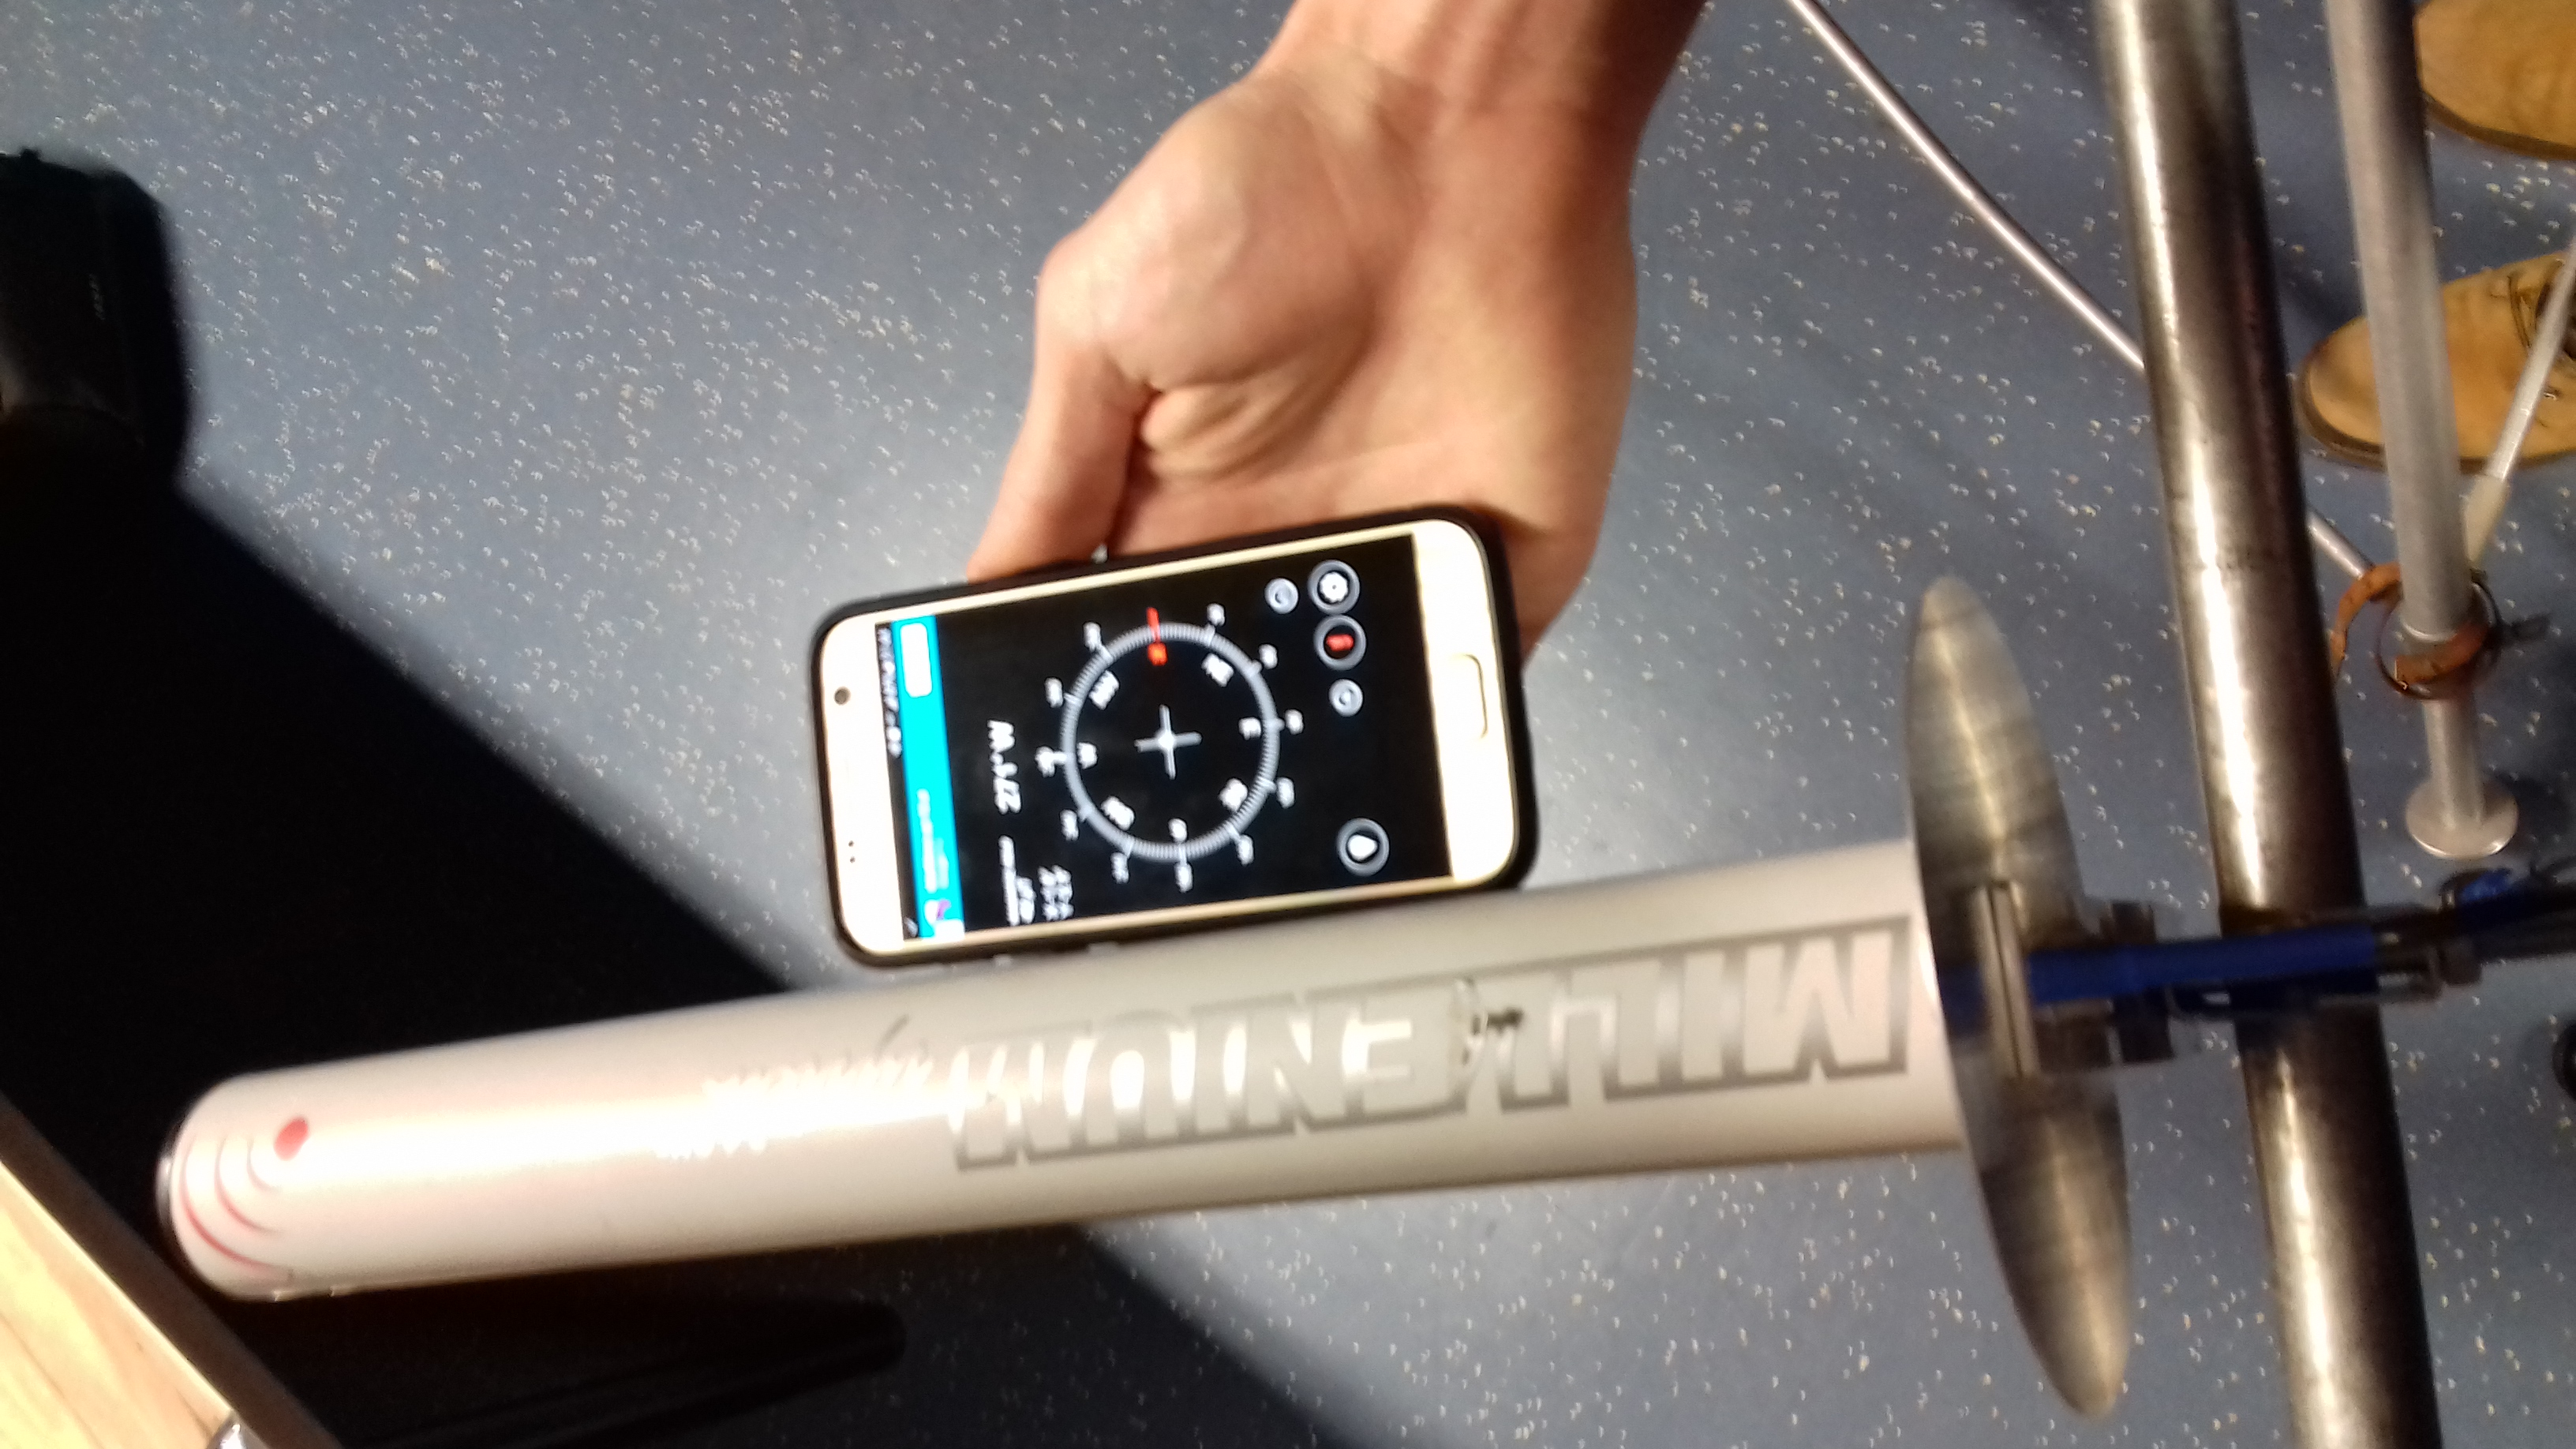
\includegraphics[width=\textwidth]{test_kierunku}
 \centering
 \caption{Sprawdzenie orientacji anteny przy pomocy zewnętrznego kompasu.}
 \label{kompas}
\end{figure}

% \todo{zjdecia w katalogu testy}

\subsection{Część radiowa}

Niemożliwe były testy bezpośrednie odbioru sygnału APRS ze względu na brak radia SDR na zadane pasmo częstotliwości, więc testy ograniczono do tych opisanych w poprzednim rozdziale.

\subsection{Podsumowanie}

Celem projektu było opracowanie mobilnej stacji do łączności radiowej z
balonem ze szczególnym zwróceniem uwagi na pasma radioamatorskie.
Stacja składa się z:
\begin{itemize}
 \item statywu z elektronicznie sterowanymi antenami,
 \item przy pomocy silników DC umożliwiających zmianę orientacji anten w płaszczyźnie azymutu i elewacji,
 \item radia programowalnego (SDR – Software
Defined Radio) do przetworzenia sygnału (wykorzystane zostało radio
będące na stanie Laboratorium Technologii Kosmicznych WEiTI),
 \item oprogramowanie SDR umożliwiające odbiór pakietów
APRS - automatycznego systemu powiadamiania o pozycji, który jest
zwykle wykorzystywany do lokalizacji balonów w misjach.
\end{itemize}

Opracowana stacja pozwalała na odbiór sygnałów w pasmach
radioamatorskich UHF (430 MHz) oraz VHF (140 MHz).
Opracowany rotor, obracający anteny w płaszczyźnie azymutu i elewacji,
może być zamontowany na rozkładanym statywie antenowym lub na
dachu samochodu (z wykorzystaniem bagażnika dachowego)
